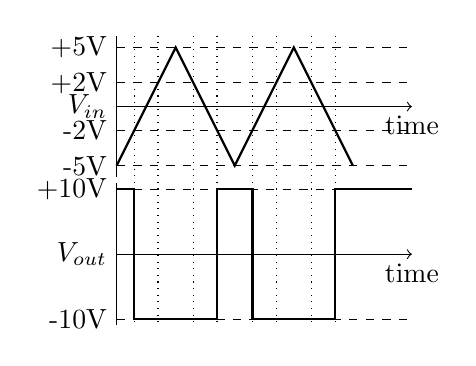
\begin{tikzpicture}[scale=0.75]
    \draw (0, 0) -- (0, 2.4); 
    \draw[->] (0, 1.2) node[left] {$V_{in}$} -- (5, 1.2) node[below] {time};
    \draw[dashed] (0, 1.6) node[left] {+2V} -- (5, 1.6);
    \draw[dashed] (0, 2.2) node[left] {+5V} -- (5, 2.2);
    \draw[dashed] (0, 0.8) node[left] {-2V} -- (5, 0.8);
    \draw[dashed] (0, 0.2) node[left] {-5V} -- (5, 0.2);
    \draw[thick] (0, 0.2) -- (1, 2.2) -- (2, 0.2) -- (3, 2.2) -- (4, 0.2);

    \foreach \i in {0,...,3} {
        \draw[dotted] (\i+0.3, 2.4) -- (\i+0.3, -2.5);
        \draw[dotted] (\i+0.7, 2.4) -- (\i+0.7, -2.5);
    }

    \draw (0, -0.1) -- (0, -2.5); 
    \draw[->] (0, -1.3) node[left] {$V_{out}$} -- (5, -1.3) node[below] {time};
    \draw[dashed] (0, -0.2) node[left] {+10V} -- (5, -0.2);
    \draw[dashed] (0, -2.4) node[left] {-10V} -- (5, -2.4);
    \draw[thick] (0, -0.2) -- (0.3, -0.2) -- (0.3, -2.4) -- (1.7, -2.4) -- (1.7, -0.2) -- (2.3, -0.2) -- (2.3, -2.4) -- (3.7, -2.4) -- (3.7, -0.2) -- (5, -0.2);
\end{tikzpicture}